\documentclass[11pt,letterpaper]{article}

\input{../../../../.config/latex/preamble_v1.tex}

\lightmode
\usetikzlibrary{decorations.pathreplacing,decorations.markings}

\title{\textbf{Math 231a Problem Set 5}}

\providecommand{\Sk}{\text{Sk}}
\providecommand{\Gr}{\text{Gr}}

\begin{document}
\maketitle

\begin{problem}\noindent
    \begin{enumerate}[(a)]
        \item Prove that complex projective space $\CP^n$ admits a CW structure in which $\Sk_{2k}\mathbb{CP}^n=\CP^k$ for any $0\leq k\leq n$. Use this to compute the homology of $\CP^n$.
        \item Endow $\Gr_2(\C^4)$ with a CW structure and use this to compute its homology.  
    \end{enumerate}
\end{problem}

\begin{solution}
    \textbf{(a)} Recall that $\CP^n$ is defined as
    \[
        \CP^n = \left(\C^{n+1} - \{0\}\right) / \{z\sim \lambda z : \lambda \neq 0\}
    .\]  
    But then letting $U(1)\subset \C$ be the unitary group and considering $S^{2k+1}$ as a subset of $\C^{k+1}$, we get isomorphisms
    \[
        \begin{aligned}
            \CP^n\cong S^{2n+1} / U(1) &\cong \left\{ \left(z, \sqrt{1-|z|^2}\right)\in \C^{n+1} : \|z\|\leq 1\right\} / \{(z,0) \sim \lambda (z,0) : \|z\|=1, \lambda \neq 0\}\\
            &\cong D^{2n} / \{z \sim \lambda z : z\in \partial D^{2n}, \lambda\neq 0\}.
        \end{aligned}
    \]
    However since $\partial D^{2n} / U(1) = S^{2n-1} / U(1) \cong \CP^{n-1}$, it follows that $\CP^n$ is created from $\CP^{n-1}$ by attaching a $2n$-cell $S^{2n-1}$ by the attachment map $\alpha : S^{2n-1} = \partial D^{2n} \to \partial D^{2n} / U(1) = \CP^{n-1}$. 
    
    \quad To summarize this CW structure, we begin with a $0$-cell, so $\CP^0=*$. Then set $\Sk_{2k+1} \CP^n = \Sk_{2k} \CP^n$ for all $0\leq k\leq n$, and $\Sk_{2k+2} \CP^n$ is the adjunction of $\Sk_{2k} \CP^n$ with $D^2n$ by the previously mentioned attachment map $\alpha : \partial D^{2n} \to \Sk_{2k} \CP^n$.
    
    \quad Now the cellular chain complex of this CW structure is 
    \[
        0 \to 0 \to \Z \to 0 \to \Z \to \cdots \to \Z \to 0 \to \Z \to 0
    .\] 
    It follows that all of these maps must be trivial, so the homology groups are:
    \[
        \boxed{H_k(\CP^n) = \begin{cases}
            \Z & 0\leq k\leq n\text{ and } k\text{ even},\\
            0 & 0\leq k\leq n\text{ and } k\text{ odd},\\
            0 & k>n.
        \end{cases}}
    \] 
        
    \textbf{(b)} For the sake of sanity, we'll use the standard CW decomposition on the Grassmanian. Recall that a \emph{Schubert symbol} is a sequence $1\leq \sigma_1 < \sigma_2 < \cdots < \sigma_k \leq n$. Each of these symbols corresponds to a $d(\sigma)$-cell in a CW decomposition of $\text{Gr}_k(\C^n)$ where $d(\sigma)=2\sum^n_{i=1}(\sigma_i - i)$. It's easy to see that there are only $6$ Schubert symbols in the case of $\text{Gr}_2(\C^4)$, each of even degree so we have the homology:
    \[
        \boxed{H_n(\text{Gr}_2(\C^4))=\begin{cases}
            \Z & n=0,2,6,8,\\
            \Z\oplus \Z & n =4,\\
            0 & \text{otherwise}.
        \end{cases}}
    \] 
\end{solution}

\begin{problem}
    Describe a functor $|\cdot | : \mathbf{ssSet} \to \mathbf{Top}$ as follows. Given a semisimplicial set $X_\bullet$, we set:
    \[
        |X_\bullet| = \frac{\coprod_n X_n\times \Delta^n}{(d_ix,y)\sim (x, d^iy)}
    .\]  
    The space $|X_\bullet|$ is called the \emph{geometric realization} of $X_\bullet$.
    \begin{enumerate}[(a)]
        \item Given a semisimplicial set $X_\bullet$ and a nonnegative integer $n\geq 0$, define a new semisimplicial set
        \[
            \text{Sk}_n X_\bullet = \begin{cases}
                X_k & k\leq n,\\
                \emptyset & k >n,
            \end{cases}    
        .\] 
        where the face maps $d_i$ are induced by those of $X_\bullet$.

        \quad Prove that $|X_\bullet|$ has a CW structure with $\text{Sk}_n|X_\bullet|=|\text{Sk}_n X_\bullet|$ and whose $n$-cells are induced by $X_n$. 

        \item Let $S_*(X_\bullet)$ denote the semisimplicial chain complex of $X_\bullet$, and let $S_*(|X_\bullet|)$ denote the singular chain complex of $|X_\bullet|$. Define a natural injection of chain complexes $S_*(X_\bullet) \hookrightarrow S_*(|X_{\bullet}|)$ and prove that it induces an isomorphism on homology.
    \end{enumerate}
\end{problem}

\begin{solution}
    \textbf{(a)} For $n=0$ we have $\Sk_0 X_\bullet = X_0$, and for $n\geq 1$ we have
    \[
        \Sk_n X_\bullet = \frac{\coprod_{k=0}^n X_k\times \Delta^k}{(d_ix,y)\sim (x, d^iy)} = \frac{\Sk_{n-1}\sqcup X_n\times \Delta^n}{(d_ix,y) \sim (x,d^iy)} = \Sk_{n-1}\cup_{\alpha_n} X_n\times \Delta^n
    \]
    where $\alpha_n : X_n\times \Delta^n \to \Sk_{n-1}$ is the canonical attachment map induced by the face maps $d_i$. Since $X_n$ is a discrete space, $\Delta^n\cong D^n$, and $d^i \Delta^n \subset \partial \Delta^n$, we have a CW structure.

    \textbf{(b)} Define the map $\alpha : S_*(X_\bullet) \hookrightarrow S_*(|X_\bullet|)$ by $\alpha_n(x)=[\{x\}\times \Delta^n]$ for any $x\in X_n$ and extending linearly. This is clearly a chain map because it commutes with the face maps, and hence the boundary operator as well. To prove that it induces an isomorphism on homology, let $\sigma : \Delta^n \to |X_\bullet|$ be a cycle. This map induces isomorphisms on homology by the cellular boundary formula.
\end{solution}

\begin{problem}
    Let $p, q \in \Z$, and let $X_{p,q}$ be the $2$-dimensional CW complex obtained by attaching two 2-cells to $S^1$ using maps of degree $p$ and $q$. Compute $\pi_1(X_{p,q})$ and $H_*(X_{p,q})$.
\end{problem}

\begin{solution}
    \quad Let's begin by calculating the fundamental group using the Seifert van-Kampen theorem. First we'll compute $\pi_1(X_p)$ where $X_p$ is the space obtained by attaching a single $1$-cell to $S^1$ using a map of degree $p$. In other words, this space is the quotient of $D^2$ by some equivalence relation $\sim_p$ on $\partial D^2$. Let $A=A_\epsilon \subset D^2$ be some subset of radius $\epsilon$, and let $B=D^2-A_{\epsilon /2}$. We can naturally identify these as subsets of $X_p$. Then applying the Siefert van-Kampen theorem and picking a suitable basepoint $x\in A\cap B$ (omitted for clarity), we get a diagram
    \begin{center}
        \begin{tikzcd}
            & {\pi_1(B)} \arrow[rd] \arrow[d, "f_B"]                             &              \\
        {\pi_1(A\cap B)} \arrow[ru, "i_B"] \arrow[rd, "i_A"'] & {\pi_1(A)*_{\pi_1(A\cap B)}\pi_1(B)} \arrow[r, dashed] & {\pi_1(X_{p,q})} \\
                    & {\pi_1(A)} \arrow[u, "f_A"'] \arrow[ru]                            &             
        \end{tikzcd}
    \end{center}
    \quad Since $A$ is contractible, it follows that $\pi_1(A,x) *_{\pi_1(A\cap B,x)} \pi_1(B,x) \cong \pi_1(B,x) / i_B(\pi_1(A\cap B,x))$. First we'll show that $\pi_1(B,x)\cong \Z$. First observe that $B$ is canonically homotopy equivalent to $S^1$ by the map which lets $\epsilon /2\to 1$, then applies $\alpha_p$, the attachment map of degree $p$. Similarly, $A\cap B$ is canonically homotopy equivalent to $S^1$. Then $i_B$ sends a generator $[\iota]$ of $\pi_1(A\cap B,x)$ to $[\alpha(\iota)]=p[\iota]$ in $\pi_1(B,x)$ so we get $\pi_1(X_{p,q},x)\cong \Z /p\Z = \Z /p$.
    
    \quad Now we can consider $X_{p,q}$ as the attachment of $X_{p}$ to $X_q$ along the image of $S^1$ in $X_p, X_q$, i.e. $X_{p,q}=(X_p\sqcup X_q) / (\alpha_p \sqcup \alpha_q)$. Let $U_p, U_q \subset X_{p,q}$ be open sets which $\epsilon$ expand $X_p$ and $X_q$ respectively. The Seifert van-Kampen theorem then gives us the pushout
    \begin{center}
        \begin{tikzcd}
            & \Z/p \arrow[rd] \arrow[d]                  &          \\
            \Z \arrow[rd, two heads] \arrow[ru, two heads] & \Z/p *_\Z \Z/q \arrow[r, dashed] \arrow[d] & \pi_1(X) \\
                        & \Z/q \arrow[ru]                            &         
            \end{tikzcd}
    \end{center}
    \quad The group presentation of $\pi_1(X)$ then becomes $\big\langle x,y \mid x^p=y^q=1, x=y \big\rangle$ which is exactly the group $\Z /\gcd(p,q)$. Here we take the convention that $\Z /0=\{1\}$ so that $\gcd(x,0)=x$ and $\gcd(0,y)=y$. So
    \[
        \boxed{\pi_1(X_{p,q})\cong \Z / \gcd(p,q).}
    \] 
    \quad Next let's compute the homology groups. Recall that our CW structure is: $X_0$ consists of a single point $v_0$, $X_1$ adds an edge $e_0$ looped at $v_0$, and $X_2$ adds two faces $f_0, f_1$ by maps $e_0^p$ and $e_0^q$ respectively. Recall that $C_n(X_{p,q})=\Z I_n$ where $I_n$ is the set of $n$-cells. Thus our chain complex is
    \begin{center}
        \begin{tikzcd}
            0 & \Z v_0 \arrow[l] & \Z e_0 \arrow[l, "\beta"'] & \Z f_0\oplus \Z f_1\arrow[l, "\alpha"'] & 0 \arrow[l]
        \end{tikzcd}
    \end{center}
    By the cellular boundary formula, we get $\beta(e_0)=0$, $\alpha(f_0)=pe_0$, and $\alpha(f_1)=qe_0$.Finally we can calculate the homology groups. $H_0(X_{p,q})=\Z /\Ima(\beta) = \Z$, $H_1(X_{p,q})=\ker(\beta) / \Ima(\alpha) = \Z /\gcd(p,q)$, and $H_2(X_{p,q})=\ker(\alpha)=\Z$ if $p,q$ are not both nonzero and $\Z\oplus \Z$ otherwise. To summarize,
    \[
        \boxed{H_n(X_{p,q})=\begin{cases}
            \Z & n=0,\\
            \Z /\gcd(p,q) & n=1,\\
            \Z & n=2\text{ and } (p,q)\neq (0,0),\\
            \Z\oplus \Z & n=2\text{ and } (p,q)=(0,0),\\
            0 & n\geq 3.
        \end{cases}}
    \]   
\end{solution}

\begin{problem}
    Compute the homology groups of the following 2-dimensional CW complexes:
    \begin{enumerate}[(a)]
        \item The quotient of $S^2$ obtained by identifying the north and south poles to a point.
        \item The space obtained from $S^2$ by first deleting the interiors of two disjoint subdisks in the
        interior of $D^2$ and then identifying all three resulting boundary circles together via homeomorphisms preserving the clockwise orientations of these circles.
    \end{enumerate}
\end{problem}

\begin{solution}
    \textbf{(a)} Let $X$ be the space. First of all, $X$ is homotopy equivalent to the torus with a disk glued into the central hole. This can be given the following CW structure: $X_0$ consists of a single point $v_0$. $X_1$ adds two circles $e_0, e_1$ at $v_0$, and $X_2$ adds two disks $f_0, f_1$, with $f_0$ glued to $e_0$ and $f_1$ glued to $e_0e_1e_0^{-1}e_1^{-1}$. (Here we use the notation $e_0e_1e_0^{-1}e_1^{-1}$ to represent the attachment map which goes around $e_0$, then $e_1$, then $e_0$ in the other direction, then $e_1$ in the other direction). We thus get the following cellular chain complex:
    \begin{center}
        \begin{tikzcd}
            0 & \Z v_0 \arrow[l] & \Z e_0\oplus \Z e_1 \arrow[l, "\beta"'] & \Z f_0\oplus \Z f_1 \arrow[l, "\alpha"'] & 0 \arrow[l]
        \end{tikzcd}
    \end{center}
    \quad Here we consider these $v_i, e_i, f_i$ as generators of $H_n(S^n)$ for the appropriate $n$. The cellular boundary formula gives $\beta(e_0)=v_0-v_0=0$ and $\beta(e_1)=v_0-v_0=0$. Similarly $\alpha(f_0)=e_0$ and $\alpha(f_1)=e_0 + e_1 - e_0 - e_1 = 0$. Then $H_0(X)=\Z / \Ima(\beta) = \Z$, $H_1(X)=\Z e_0 \oplus \Z e_1 / \Z e_0 = \Z$, and $H_2(X)=\Z e_1 / 0 = \Z$. Thus
    \[
        \boxed{H_n(X)=\begin{cases}
            \Z& n=0,1,2,\\
            0& n\geq 3.
        \end{cases}}
    \]    

    \textbf{(b)} Let $X$ be the space. Let's give the following CW structure to $X$:

    \begin{center}
        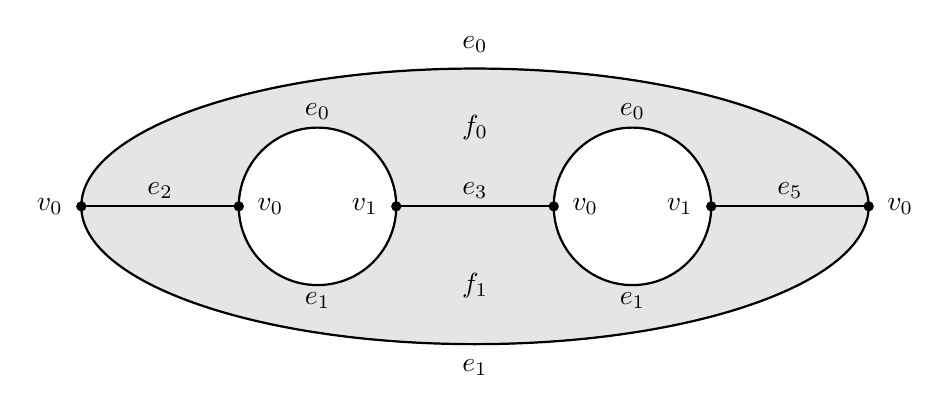
\begin{tikzpicture}
            \draw[fill=gray!20] (0,0) ellipse (5.0 and 1.75);
            \draw[fill=white] (2,0) circle (1);
            \draw[fill=white] (-2,0) circle (1);

                \node[] () at (-2,1.2) {$e_0$};
                \node[] () at (-2,-1.2) {$e_1$};
                \draw[thick] (-2,0) circle (1);
                \node[] () at (2,1.2) {$e_0$};
                \node[] () at (2,-1.2) {$e_1$};
                \draw[thick] (2,0) circle (1);
                \node[] () at (0,0.2) {$e_3$};
                \draw[thick] (-1,0) -- (1,0);
                \node[] () at (-4,0.2) {$e_2$};
                \draw[thick] (-5,0) -- (-3,0);
                \node[] () at (4,0.2) {$e_5$};
                \draw[thick] (5,0) -- (3,0);
                \node[] () at (0,2.05) {$e_0$};
                \draw[thick] (5,0) arc(0:180:5 and 1.75) (-5,0);
                \node[] () at (0,-2.05) {$e_1$};
                \draw[thick] (5,0) arc(0:180:5 and -1.75) (-5,0);

                \node[] () at (0,1) {$f_0$};
                \node[] () at (0,-1) {$f_1$};

                \node[] () at (-1.4,0) {$v_1$};
                \draw[thick, fill] (-1,0) circle (0.05);
                \node[] () at (1.4,0) {$v_0$};
                \draw[thick, fill] (1,0) circle (0.05);
                \node[] () at (-2.6,0) {$v_0$};
                \draw[thick, fill] (-3,0) circle (0.05);
                \node[] () at (2.6,0) {$v_1$};
                \draw[thick, fill] (3,0) circle (0.05);
                \node[] () at (-5.4,0) {$v_0$};
                \draw[thick, fill] (-5,0) circle (0.05);
                \node[] () at (5.4,0) {$v_0$};
                \draw[thick, fill] (5,0) circle (0.05);
        \end{tikzpicture}
    \end{center}
    So $X_0$ consists of two $0$-cells, $X_1$ adds five $1$-cells, and $X_2$ adds two $2$-cells. This gives us the chain complex 
    \begin{center}
        \begin{tikzcd}
            0 & \Z^2 \arrow[l] & \Z^5 \arrow[l, "\beta"'] & \Z^2 \arrow[l, "\alpha"'] & 0 \arrow[l]
        \end{tikzcd}
    \end{center}
    with boundary maps $\alpha, \beta$ given by:
    \[
        \begin{aligned}
            \beta(e_0) &= v_1 - v_0 \quad\quad\quad\quad &\alpha(f_0) = e_0+e_2+e_3+e_4\\
            \beta(e_1) &= v_1 - v_0 \quad &\alpha(f_1) = e_1+e_2+e_3+e_4\\
            \beta(e_2) &= 0\quad &\\
            \beta(e_3) &= v_1 - v_0\quad &\\
            \beta(e_4) &= 0\quad &\\
        \end{aligned}
    \]
    Then it's fairly easy to see by calculating kernels and images of these maps that
    \[
        \boxed{H_n(X) = \begin{cases}
            \Z &n=0,\\
            \Z\oplus \Z & n=1,\\
            0 & n\geq 2.\\
        \end{cases}}
    \]  
\end{solution}

\end{document}